%--------------------------------------------%
% Template Beamer para Apresentações da UFRN %
% by alcemygvseverino@gmail.com              %
% Baseado em MIT Beamer Template	     %
% versao 1.1				     %
% Atualizado em 14/05/2016		     %
% Modificado em 20/05/2017 		     %
%    José W. R. Pereira - IFSP
%--------------------------------------------%
\documentclass[handout,t]{beamer}
% Para alterar a linguagem do documento
\usepackage[portuges]{babel}
% Para aceitar caracteres especias deretamente do teclado
\usepackage[utf8]{inputenc}
% Para seguir as normas da ABNT de citacao e referencias
\usepackage[alf]{abntex2cite}
% Para incluir figuras
\usepackage{graphicx}
% Para melhor ajuste da posisao das figuras
\usepackage{float}
% Para ajustar as dimensoes do layout da pagina
\usepackage{geometry}
% Para formatar estrutura e informacoes de formulas matematicas
\usepackage{amsmath}
% Para incluir simbolos especiais em formulas matematicas
\usepackage{amssymb}
% Para incluir links nas referencias
\usepackage{url}
% Para incluir paginas de documentos .pdf externos
\usepackage{pgfpages}
% Para ajustar o estilo dos contadores
\usepackage{enumerate}
% Para modificar a cor do texto
\usepackage{color}
% Para incluir condicoes
\usepackage{ifthen}
% Para colocar legendas em algo que nao e float
\usepackage{capt-of}
% Para utilizar biblioteca de construcao de figuras
\usepackage{tikz}
% Para utilizar duas figuras lado a lado
\usepackage{subfig}
% Para utilizar biblioteca de simbolos matemáticos (Laplace)
\usepackage{mathrsfs}
% Para utilizar a cor e as colunas em uma tabela
\usepackage{colortbl}
\usepackage{multirow}


% Para definir o tema do slide
\usetheme{Berlin}
% Para difinir cores e background
\usecolortheme{ufrn}
% Para numerar as figuras
\setbeamertemplate{caption}[numbered]

% Título
\title[]{
Controle de Sistema Dinâmico Utilizando Lógica Paraconsistente Anotada Evidencial $E\tau$(LPA$E\tau$)}
% Data
\date{01 de Agosto de 2018}
% Autores
\author[José W. R. Pereira]
{
	José William Rodrigues Pereira\inst{1}\\
	\vspace{0.25cm}
	Orientador: Profº Dr. Tarcisio Fernandes Leão\inst{2}
}
% Instituto
\institute[INSTITUTO]
{
	\inst{1}%
	\url{josewrpereira@gmail.com}\\
	\vspace{0.25cm}
	\inst{2}%
	\url{leao@ifsp.edu.br}
\
}
% Logo do canto inferior direito
\pgfdeclareimage[height=0.7cm]{logo_IFSP}{figuras/logo_IFSP}
\logo{
	\vspace*{-0.25cm}
	\pgfuseimage{logo_IFSP}
	\hspace*{-0.05cm}}


\begin{document}
% Sumário
\frame{\titlepage}
\section[]{}
\begin{frame}{Sumário}
	\tableofcontents
\end{frame}

% Introducao
\section{Introdução}
\begin{frame}{Introdução}

%\centering
%\begin{minipage}{0.8\textwidth}

\begin{block}{Lógica Paraconsistente \tiny \cite{JoaoInacio}}
\begin{itemize}
\item Ferramenta promissora para tomada de decisão;
\item Robótica, Automação Industrial, IA, Logística, etc.
\end{itemize}
\end{block}

\begin{alertblock}{Ideia de uso da Lógica Paraconsistente \tiny \cite{JISF2011}}
\begin{itemize}
\item Conjunto de axiomas e regras de inferência;
\item Objetiva representar formalmente um raciocínio válido.
\end{itemize}
\end{alertblock}

%\end{minipage}
%\end{frame}


\end{frame}


%%%%%%%%%%%%%%%%%%%%%%%%%%%%%%%%%%%%%%% Objetivo
\begin{frame}{Objetivo(s)}
\begin{exampleblock}{Geral}
Estudar a LPA2v e desenvolver um algoritmo que possa ser embarcado para atuar no controle dinâmico de um sistema físico.
\end{exampleblock}

\begin{alertblock}{Específicos}
\begin{itemize}
\item Construir um sistema físico para o controle de velocidade em um motor CC.
\item Implementar o algorítmo da LPA2v e criar uma biblioteca.
\item Desenvolver a malha de controle do sistema físico proposto utilizando o algorítmo da LPA2v.
\end{itemize}
\end{alertblock}

\end{frame}



%%%%%%%%%%%%%%%%%%%%%%%%%%%%%%%%%%%%%%% Lógica Clássica
\begin{frame}{Lógica Clássica}
\begin{block}{A origem \tiny \cite{JoaoInacio}}
Grécia Antiga : \emph{Tópicos} de Aristóteles  340 a.C.
\end{block}
\begin{block}{Princípios da Lógica \tiny \cite{JoaoInacio}}

\begin{enumerate}
\item Princípio de Identidade: 
    \begin{math}
	A \rightarrow A 
	\textrm{ ou } 
	\forall x(x=x);
    \end{math}

\item Princípio do Terceiro Excluído:
    \begin{math}
	A \vee \neg A
	\textrm{ ou }
	\forall x(Ax \vee \neg Ax);
    \end{math}

\item Princípio da Não Contradição: 
    \begin{math}
	\neg (A \wedge \neg A)
	\textrm{ ou }
	\forall x\neg(Ax \wedge \neg Ax).
    \end{math}

\end{enumerate}


\end{block}
\end{frame}

%%%%%%%%%%%%%%%%%%%%%%%%%%%%%%%%%%%%%%% Lógica Paraconsistente
\begin{frame}{Lógica Paraconsistente}

\begin{block}{Criadores \tiny \cite{DecioKrause}}
\begin{itemize}
\item Newton Carneiro Affonso da Costa (1929-presente data)
\item Stanislaw Jaskiwski (1906-1965)
\end{itemize}
\end{block}

\begin{block}{Desenvolvimento: Costa, Subrahmanian e Vago \tiny \cite{DecioKrause}}
\begin{itemize}
\item Lógica Paraconsistente Anotada
\item extensão a uma Lógica de Predicados Paraconsistente Anotada de primeira ordem 
\end{itemize}
\end{block}

\end{frame}

%%%%%%%%%%%%%%%%%%%%%%%%%%%%%%%%%%%%%%% Lógica Paraconsistente Anotada
\begin{frame}{Lógica Paraconsistente Anotada de Anotação com dois valores (LPA2v) \tiny \cite{JoaoInacio}}

\begin{block}{
\centering 
$\tau = \{ ( \mu , \lambda ) \mid \mu ,\lambda \in [0,1] \subset \Re \}$
}
\end{block}
\vspace{0.4cm}
\begin{minipage}{0.40\linewidth}
\begin{figure}[!htb]
%\caption{Reticulado finito de Hasse}
\center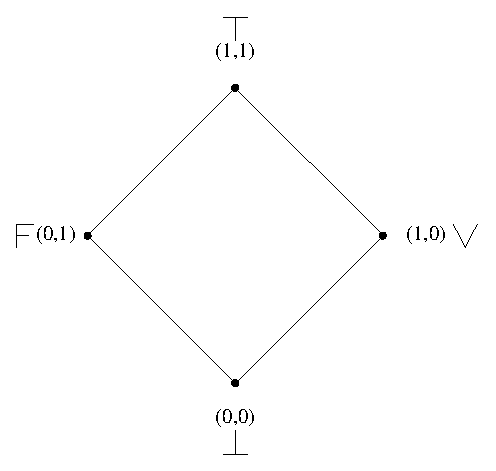
\includegraphics[scale=0.6]{./imagens/C421reticuladoHasse.eps}
\label{fig:reticuladoHasse}
%%%{\small Fonte: \cite{JoaoInacio} }
\end{figure}
\end{minipage}
\begin{minipage}{0.55\linewidth}
\center
\begin{itemize}
\item $(0,0) = \bot \Rightarrow $ Paracompleto;
\item $(0,1) = F \Rightarrow $ Falso;
\item $(1,1) = \top \Rightarrow $ Contradição;
\item $(1,0) = V \Rightarrow $ Verdade.
\end{itemize}
\end{minipage}

\end{frame}
%%%%%%%%%%%%%%%%%%%%%%%%%%%%%%%%%%%%%%% Proposição
\begin{frame}{A Proposição}
\vspace{1cm}

\begin{block}{}
\center
Para toda \textbf{proposição $P$} há um par de valores, \\
chamada de \textbf{anotação}, \textbf{$(\mu , \lambda )$}, onde \\
$\mu$ é o \textbf{grau de evidência favorável} e \\
$\lambda $ é o \textbf{grau de evidência desfavorável}, \\
representada como  \textbf{$P_{( \mu , \lambda )}$ }.
\end{block}

\end{frame}


%%%%%%%%%%%%%%%%%%%%%%%%%%%%%%%%%%%%%%% Quadrado Unitário no Plano Cartesiano
\begin{frame}{Quadrado Unitário no Plano Cartesiano}

\begin{block}{ \centering   $(\mu, \lambda ) \leftrightarrow (x,y) $ } \end{block}
\vspace{1cm}
\begin{minipage}{0.40\linewidth}
\begin{figure}[!htb]
%\caption{Representação do reticulado no quadrado unitário no plano cartesiano}
\center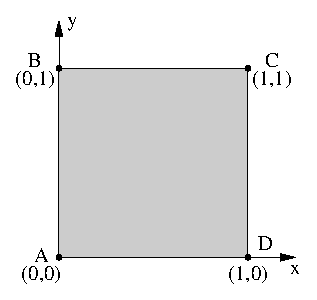
\includegraphics[scale=1.0]{./imagens/C422qupc.eps}
\label{fig:reticuladoQUPC}
%%%{\small Fonte: \cite{JoaoInacio} }
\end{figure}
\end{minipage}
\begin{minipage}{0.55\linewidth}
\center
\begin{itemize}
\item $A: (0,0) = \bot \Rightarrow $ Paracompleto;
\item $B: (0,1) = F \Rightarrow $ Falso;
\item $C: (1,1) = \top \Rightarrow $ Contradição;
\item $D: (1,0) = V \Rightarrow $ Verdade.
\end{itemize}
\end{minipage}

\end{frame}

%%%%%%%%%%%%%%%%%%%%%%%%%%%%%%%%%%%%%%% Reta Perfeitamente Definida
\begin{frame}{Reta Perfeitamente Definida}
\begin{block}{ \centering   $(\mu, \lambda ) \leftrightarrow (x,y) $ } \end{block}
\vspace{1cm}
\begin{minipage}{0.50\linewidth}
\begin{figure}[!htb]
%\caption{Representação da Reta Perfeitamente Definida}
\center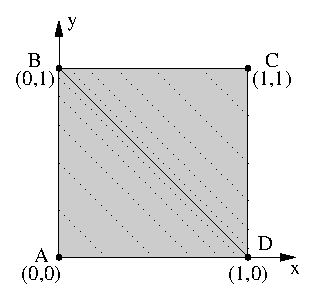
\includegraphics[scale=1.0]{./imagens/C424retaPerfeitamenteDefinida.eps}
%\label{fig:retaPerfeitamenteDefinida}
%%%{\small Fonte: \cite{JoaoInacio} }
\end{figure}
\end{minipage}
\begin{minipage}{0.45\linewidth}

\begin{itemize}
\item $\mu + \lambda = 1$
\item $\mu + \lambda - 1 = 0$
\item Grau de contradição
  \begin{itemize}
    \item $G _{ct} = \mu + \lambda - 1$
    \item $-1 \leqslant G _{ct} \leqslant 1$
  \end{itemize}
\end{itemize}
\end{minipage}

\end{frame}

%%%%%%%%%%%%%%%%%%%%%%%%%%%%%%%%%%%%%%% Reta Perfeitamente Indefinida
\begin{frame}{Reta Perfeitamente Indefinida}
\begin{block}{ \centering   $(\mu, \lambda ) \leftrightarrow (x,y) $ } \end{block}
\vspace{1cm}
\begin{minipage}{0.50\linewidth}
\begin{figure}[!htb]
%\caption{Representação da Reta Perfeitamente Indefinida}
\center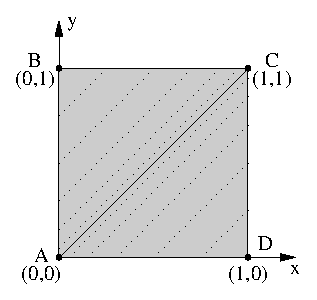
\includegraphics[scale=1.0]{./imagens/C426retaPerfeitamenteIndefinida.eps}
%\label{fig:retaPerfeitamenteDefinida}
%%%{\small Fonte: \cite{JoaoInacio} }
\end{figure}
\end{minipage}
\begin{minipage}{0.45\linewidth}

\begin{itemize}
\item $\mu - \lambda = 0$
\item Grau de certeza
  \begin{itemize}
    \item $G _{c} = \mu - \lambda$
    \item $-1 \leqslant G _{c} \leqslant 1$
  \end{itemize}
\end{itemize}
\end{minipage}

\end{frame}

%%%%%%%%%%%%%%%%%%%%%%%%%%%%%%%%%%%%%%% Representação do reticulado
\begin{frame}{\small{Representação do Reticulado da LPA2v subdividido em 12 regiões}}
\vspace{1cm}
\begin{minipage}{0.50\linewidth}
\begin{figure}[!htb]
%\caption{Representação dos valores de controle}
\center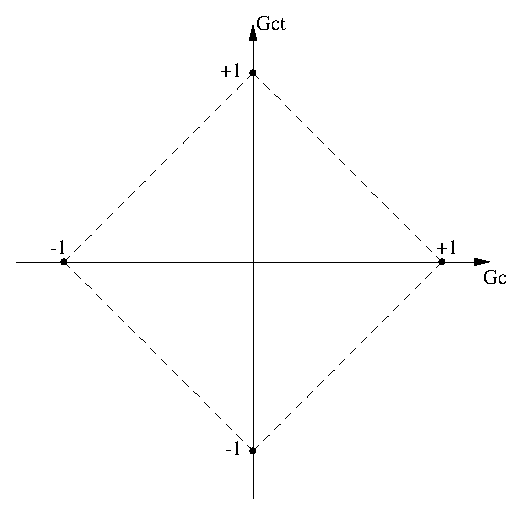
\includegraphics[scale=0.65]{./imagens/C428retasgcgct.eps}
\end{figure}
\end{minipage}
\begin{minipage}{0.45\linewidth}
\begin{figure}[!htb]
\center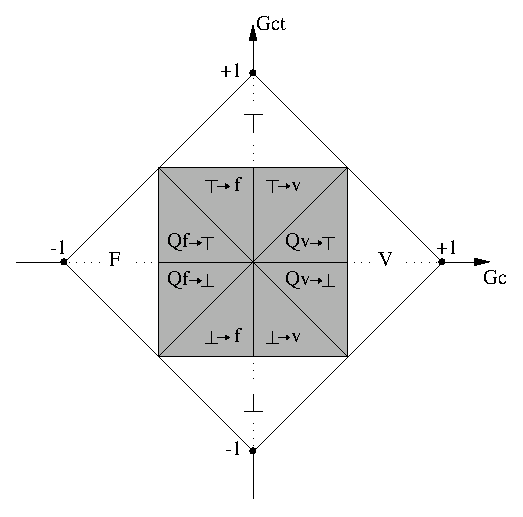
\includegraphics[scale=0.65]{./imagens/C430gcgct.eps}
%\caption{Representação do reticulado da LPA2v subdividido em 12 regiões}
\label{fig:reticuladoLPA2v}
\end{figure}
\end{minipage}

\end{frame}




% Desenvolvimento
\include{tex/desenvolvimento/desenvolvimento}

% Metodologia
\section{Metodologia}

\begin{frame}{Metodologia}
A construção dos sistemas de controle de acordo com \cite{dorf2011modern} passam basicamente por três etapas:

\vspace{1cm}

\begin{enumerate}
\item Estabelecer objetivos: 
    	\begin{itemize}
	\item variáveis de controle;
	\item especificação do sistema.
	\end{itemize}
\item Configuração do sistema
	\begin{itemize}
	\item Modelo matemático do Sistema.
	\end{itemize}
\item Controle:
	\begin{itemize}
	\item Desenvolvimento;
	\item Simulação;
	\item Análise.
	\end{itemize}
\end{enumerate}
\end{frame}




%%%%%%%%%%%%%%%%%%%%%%%%%%%%%%%%%%%%%%% Construção do Sistema Físico
\begin{frame}{Construção do Sistema Físico}

\begin{figure}[!htb]
\subfloat[Placa de desenvolvimento]{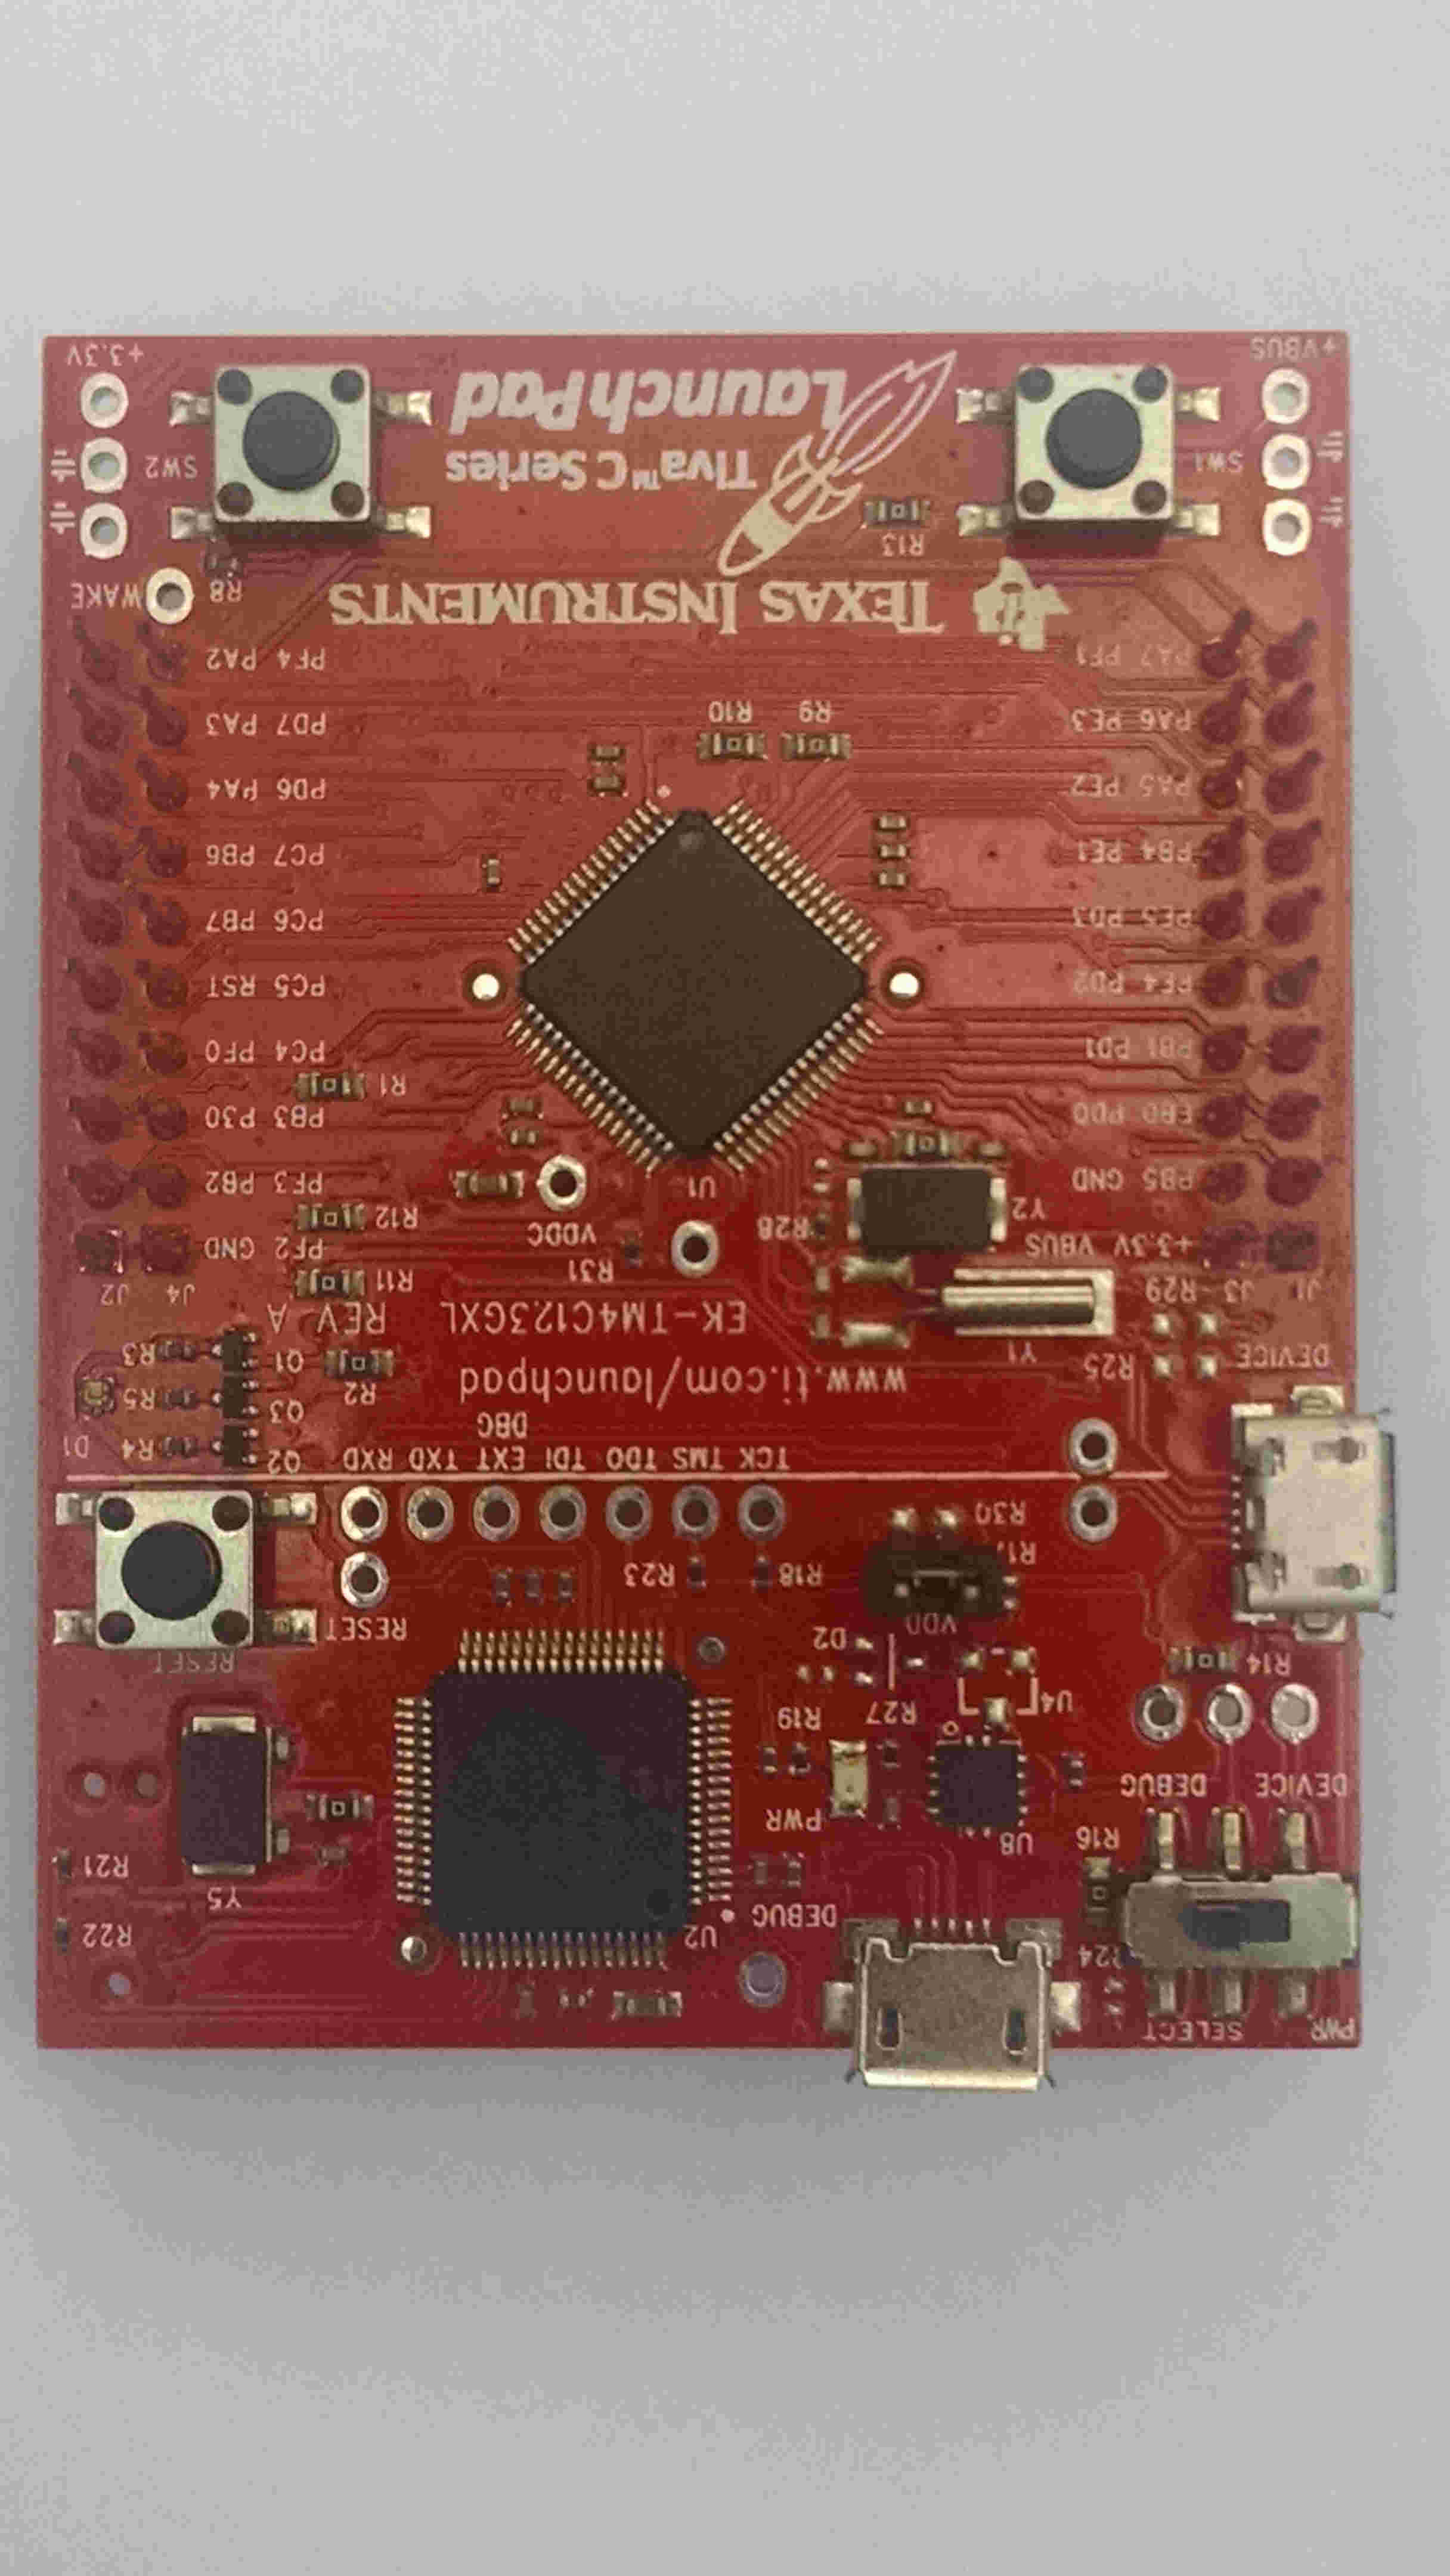
\includegraphics[scale=0.05, angle=180, clip=true, trim=0 750 60 500]{./imagens/uC-ARM.jpg}}
\subfloat[Motor CC]{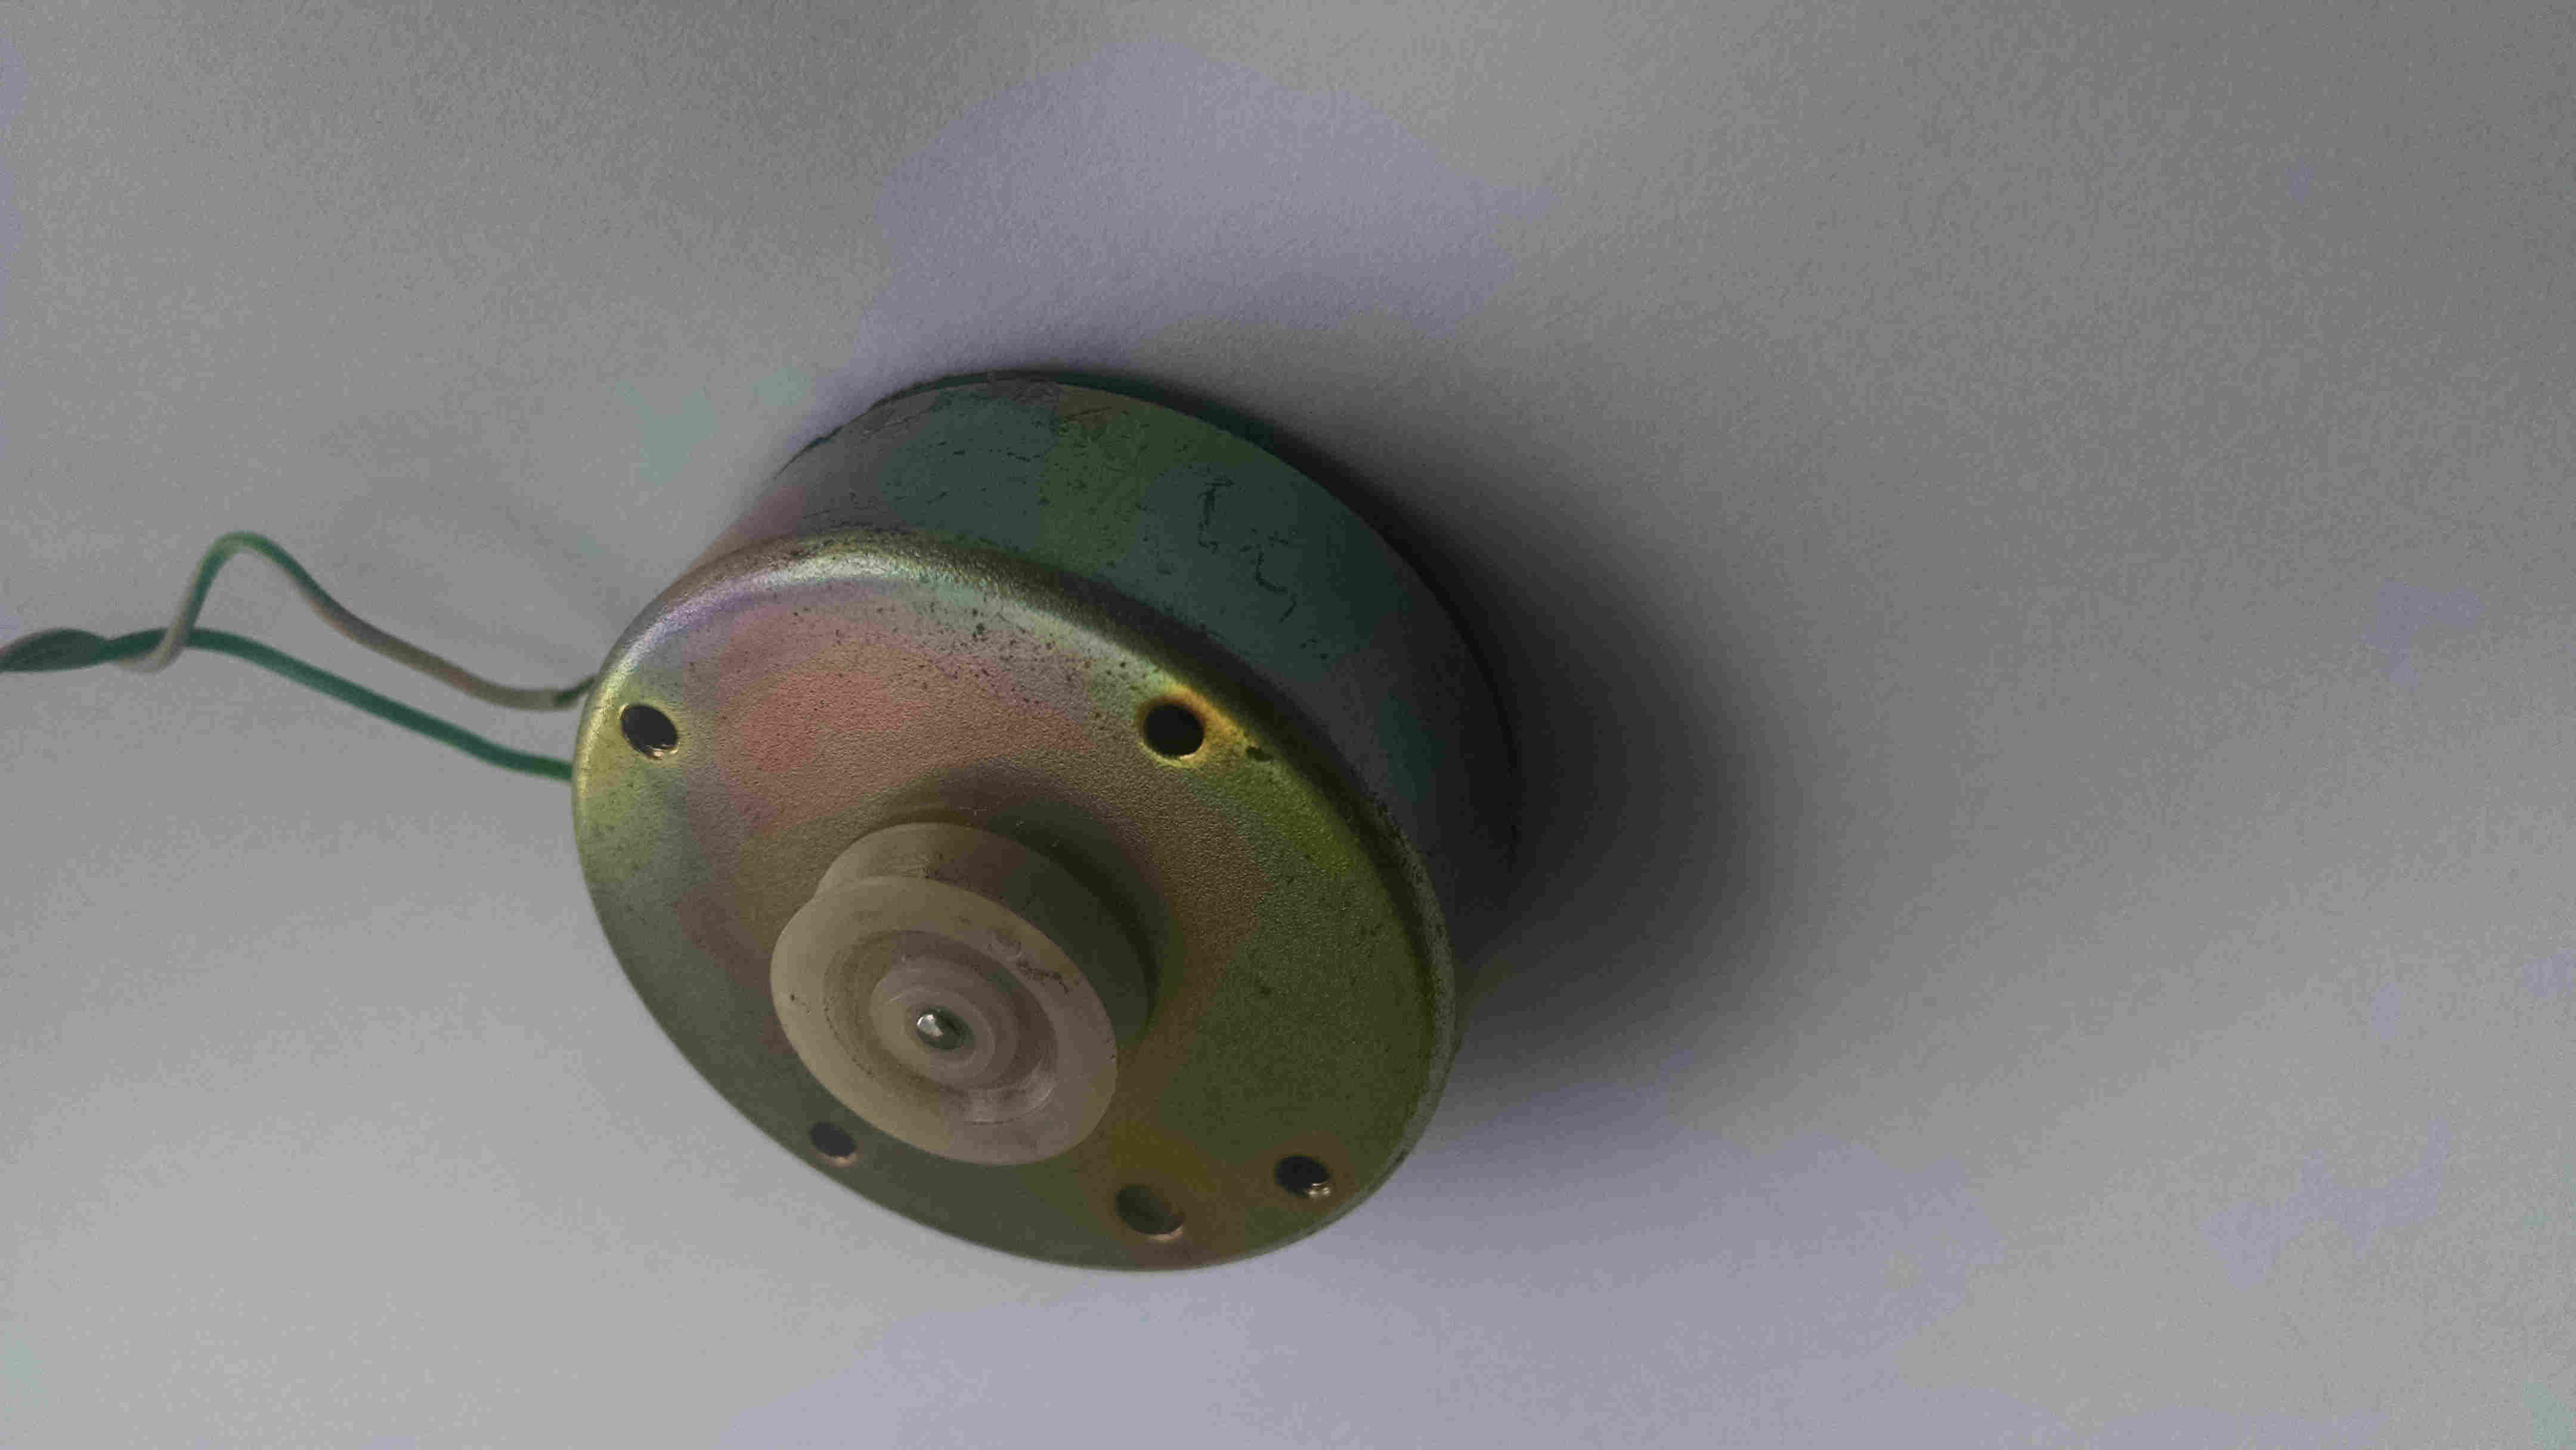
\includegraphics[scale=0.06, angle=180, clip=true, trim=700 200 1500 300]{./imagens/motorDC.jpg}}
\end{figure}

\end{frame}


%%%%%%%%%%%%%%%%%%%%%%%%%%%%%%%%%%%%%%% Estabelecer Objetivos
\begin{frame}{Estabelecer Objetivos}

\begin{itemize}
\item Variável Controlada : Velocidade de rotação do motor;
\item Variável Manipulada : Tensão aplicada no motor através de Modulação por largura de Pulso (\emph{Pulse Width Modulation - PWM});
\item Obter um modelo do sistema físico;
\item Erro aceitável para o modelo matemático de no máximo 5\%.
\end{itemize}

\end{frame}


%%%%%%%%%%%%%%%%%%%%%%%%%%%%%%%%%%%%%%% Sistema construido
\begin{frame}{Sistema construído}

\begin{figure}[!htb]
\subfloat[Sensor de rotação]{ 	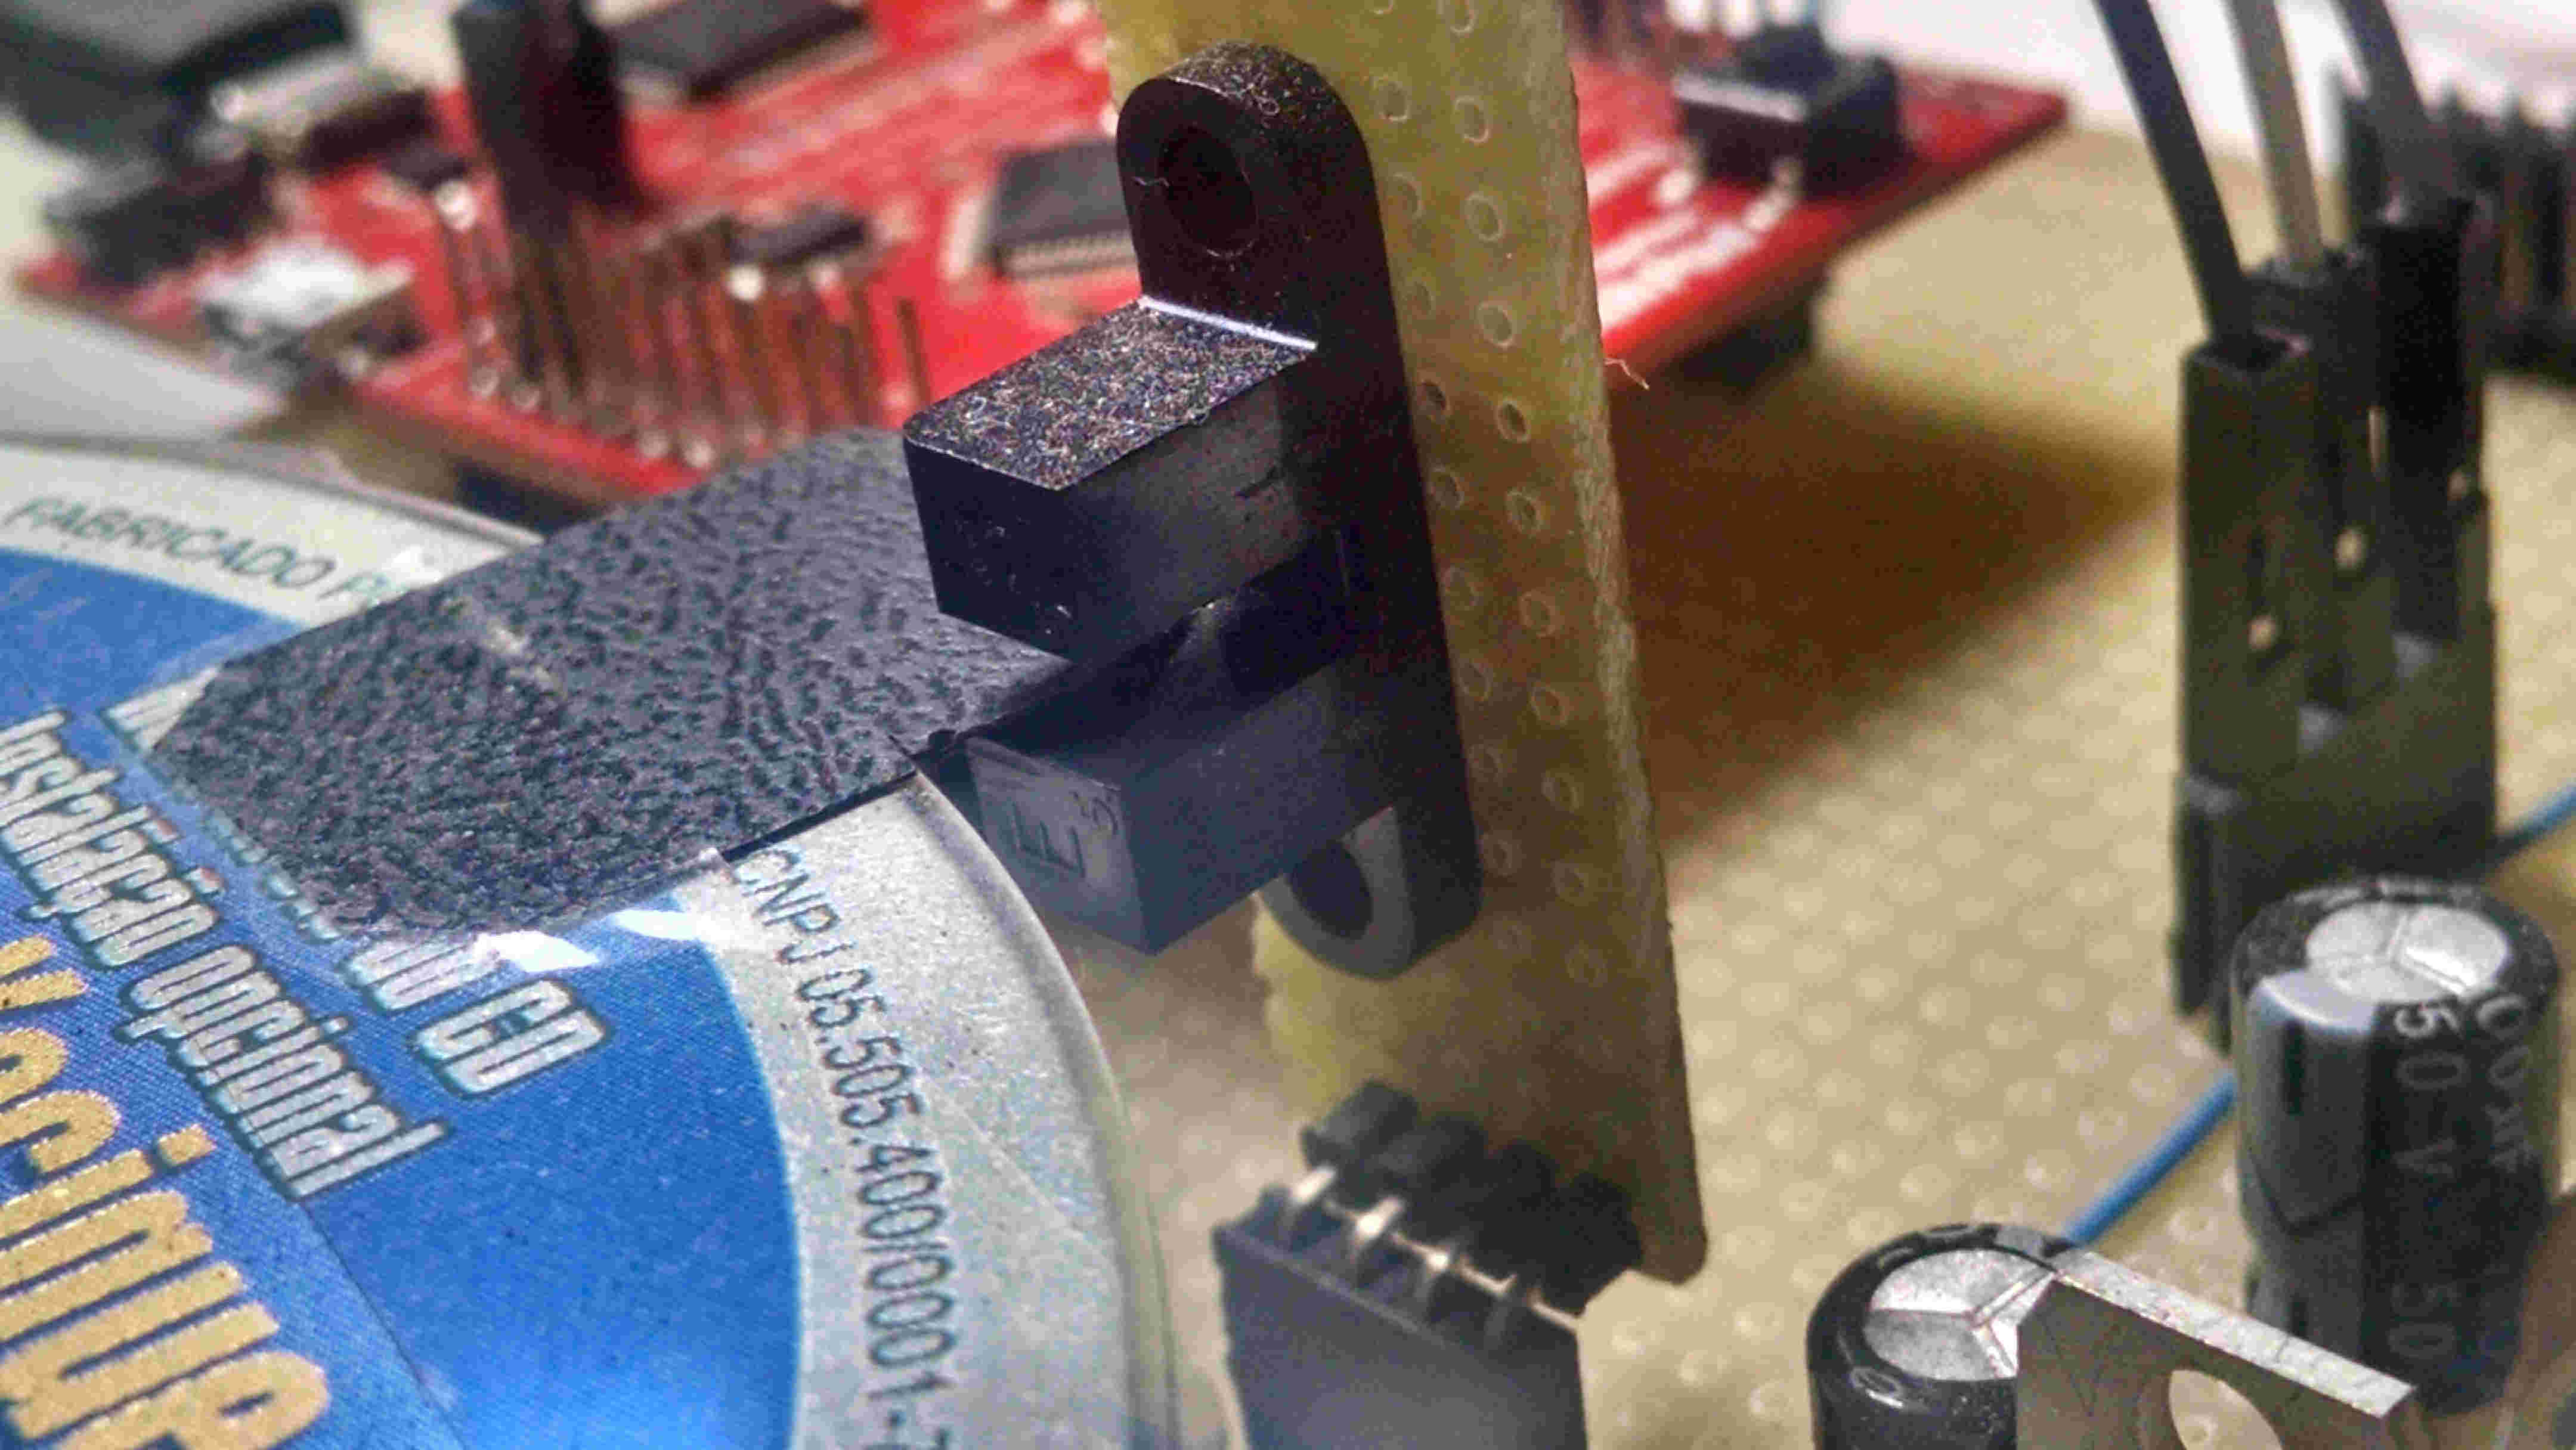
\includegraphics[scale=0.05, angle=0, clip=true, trim=300 200 1200 200]{./imagens/discoSensor.jpg} 	}
\subfloat[Planta de testes]{ 	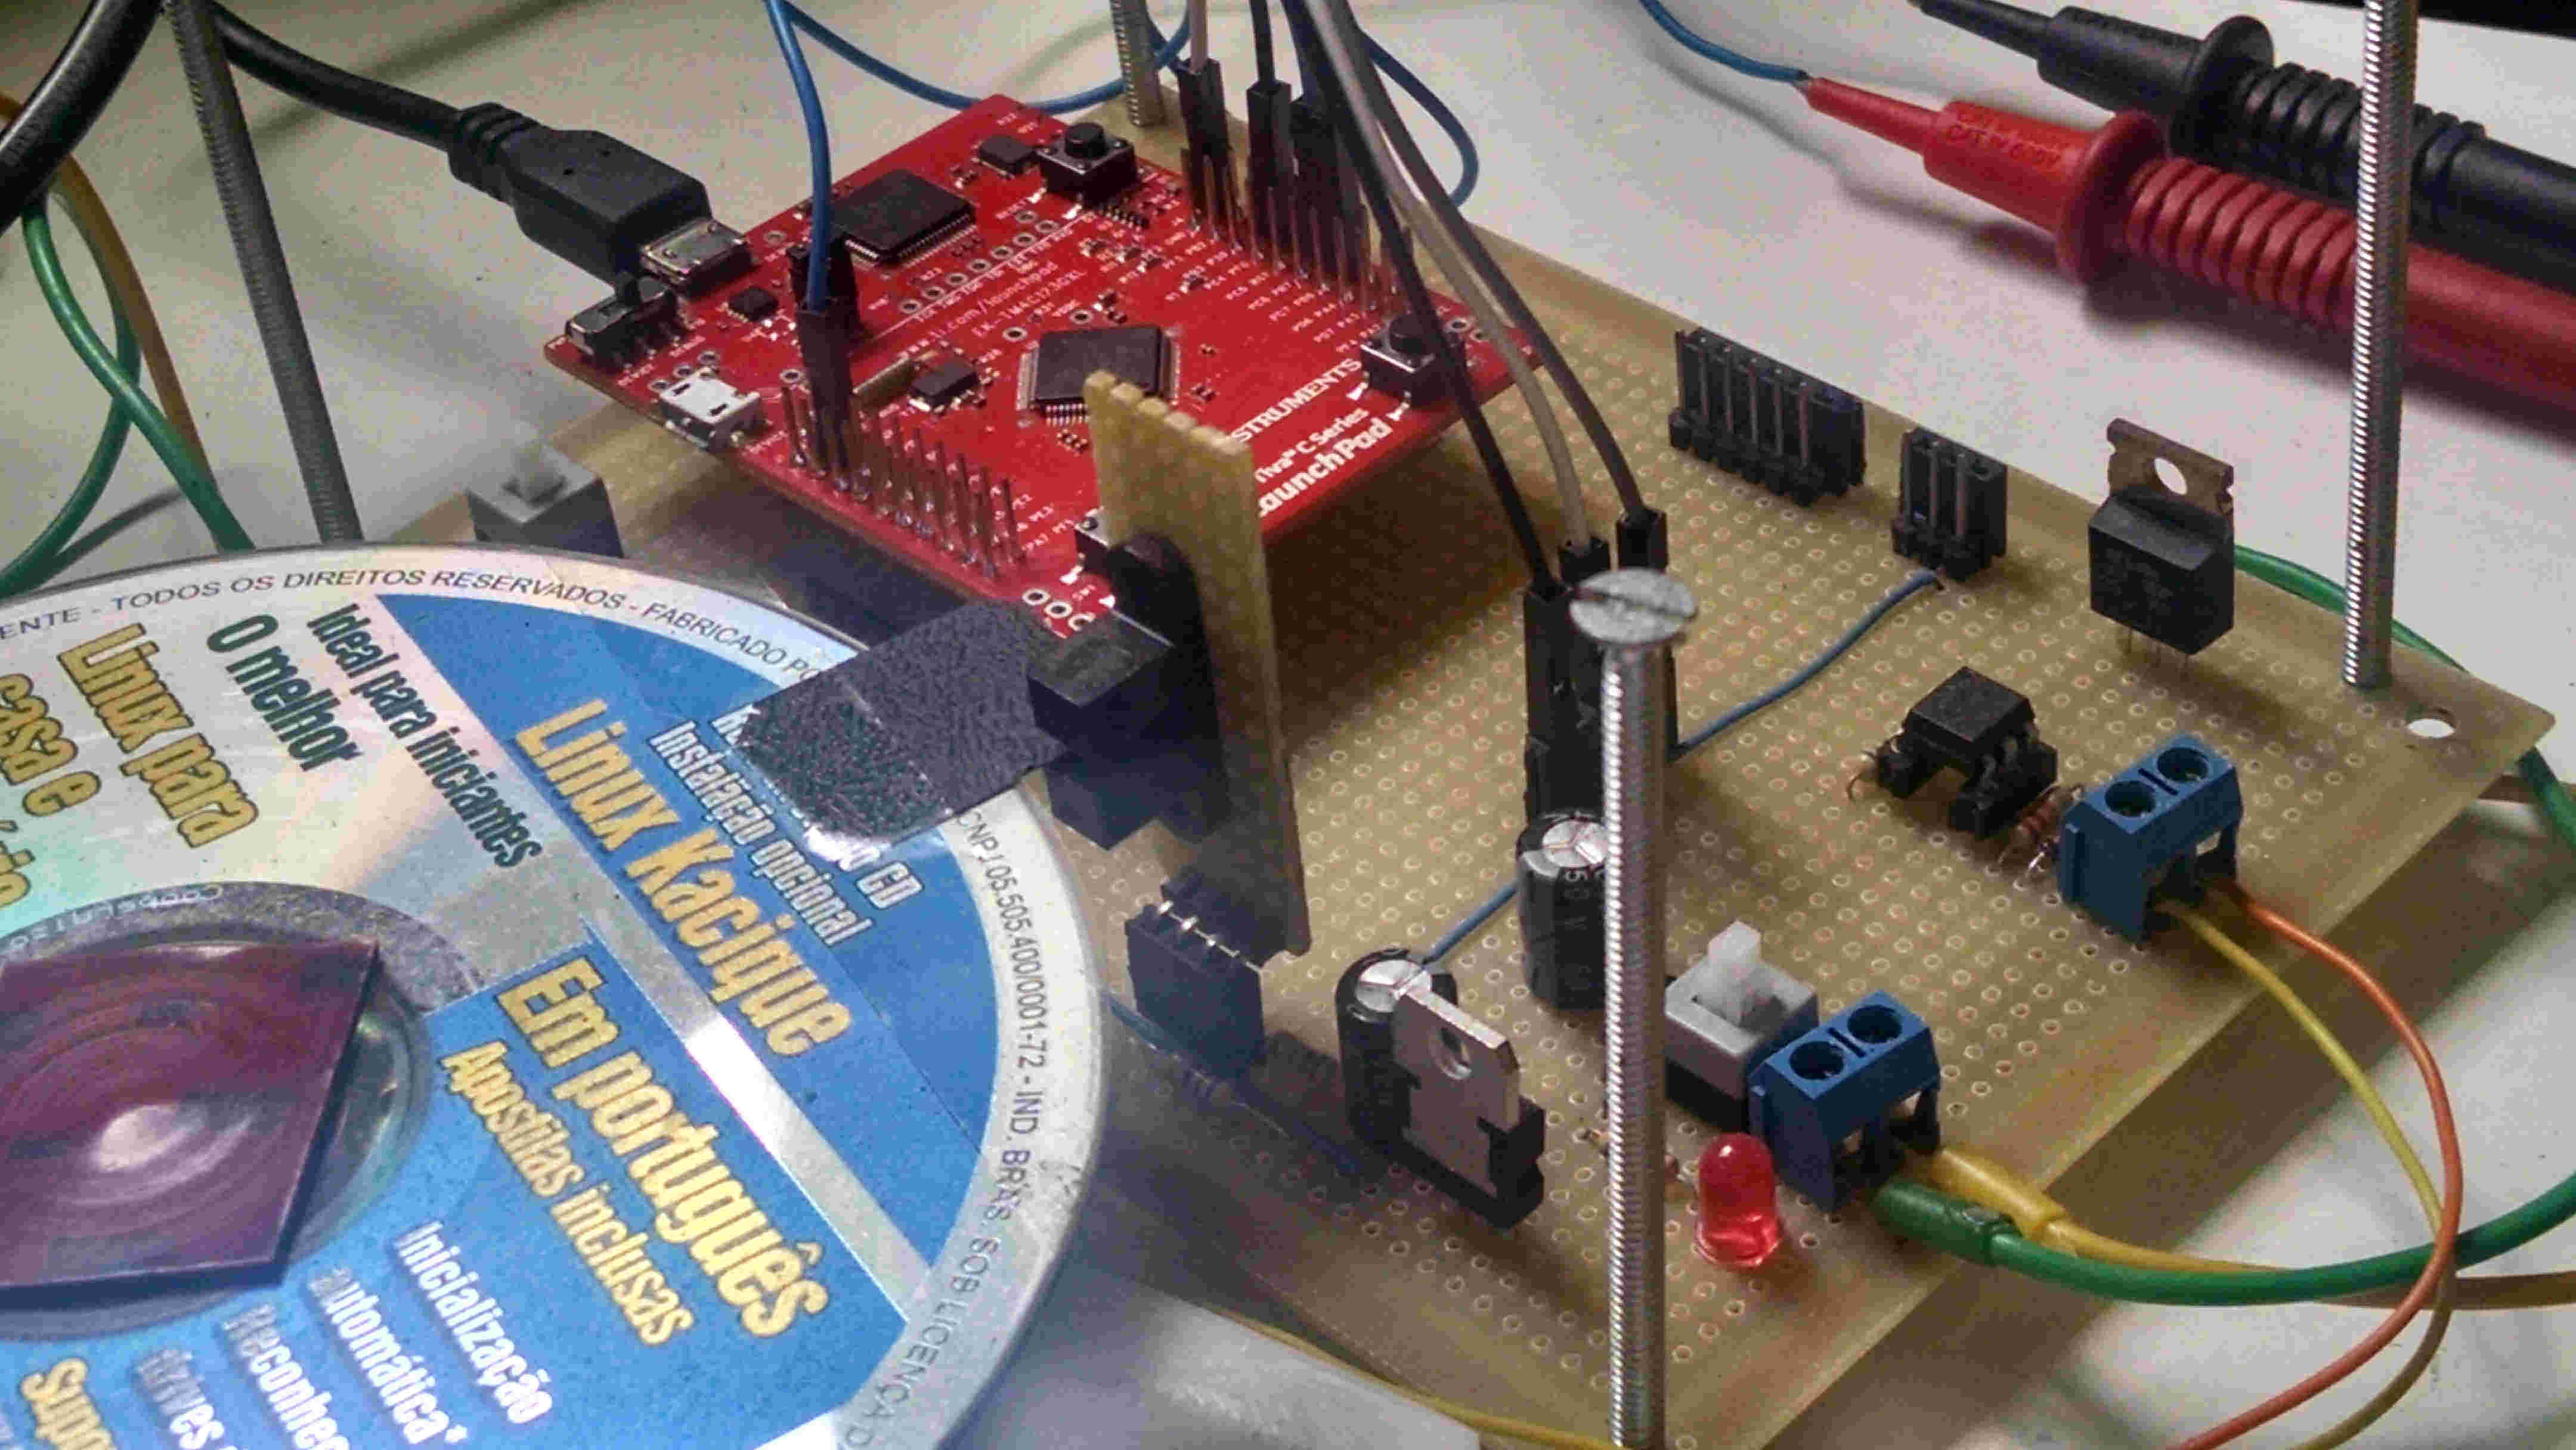
\includegraphics[scale=0.05, angle=0, clip=true, trim=300 200 400 200]{./imagens/discoSensorGeral.jpg} 	}

\end{figure}

\end{frame}

%%%%%%%%%%%%%%%%%%%%%%%%%%%%%%%%%%%%%%% Estabelecer uma meta
\begin{frame}{Estabelecer uma meta para o controle em malha fechada \tiny \cite{dorf2011modern}}
\vspace{-0.3cm}
\begin{itemize}
\item Tempo de subida: $\leqslant 20\%$ \small{do tempo de subida em malha aberta};
\item Sobressinal: $\leqslant$ 10\%;
\item Erro de regime estacionário: $\leqslant$ 5\%.
\end{itemize}

\vspace{-0.2cm}

\begin{figure}[!htb]
\centering
%\caption{Gráfico da função Resposta}
\begin{tikzpicture}[scale=0.70]
\draw [lightgray, dashed](0,0) grid (8.8,5.8);

\draw [->] (0,0) -- (9,0); 
\draw [fill] (0,6.2) -- (-0.1, 5.8) -- (0.1,5.8) -- (0,6.2);

\draw [->] (0,0) -- (0,6);
\draw [fill] (9.2,0) -- (8.8,0.1) -- (8.8,-0.1)--(9.2,0.0);

\draw [purple, ->] (7.5,4.0) -- (7.5,4.6); 
\draw [purple, fill] (7.5,4.8) -- (7.4,4.5) -- (7.6,4.5)--(7.5,4.8);

\draw [purple, ->] (7.5,6.0) -- (7.5,5.2); 
\draw [purple, fill] (7.5,5.0) -- (7.4,5.3) -- (7.6,5.3)--(7.5,5.0);

\node at (9.0,-0.5) {$t$};
\node at (0.2,6.5) {$r(t)$};

\draw [blue, ultra thick] (0.0,5.0) -- (9.0,5.0);
\draw [blue, ultra thick] (0.0,0.0) -- (0.0,5.0);

\draw [red, ultra thick] (0.0,0.0) to [out= 85, in=180] (3,5.4);
\draw [red, ultra thick] (3.0,5.4) to [out=  0, in=180] (6,4.8);

\draw [purple, ultra thick] (6,4.8) -- (9,4.8);

\node at (-1.1,5.4)[blue]{{Resposta}};
\node at (-1.1,4.8)[blue]{{desejada}};
\node at (2.0,2.2)[red]{{Resposta}};
\node at (2.0,1.6)[red]{{transiente}};
\node at (3.0,6.0)[red]{{Sobressinal}};
\node at (7.0,3.4)[purple]{{Erro de Regime Estacionário}};

\end{tikzpicture} 
\label{fig:funcaoResposta}

%{\small Fonte: \cite{dorf2011modern} }
\end{figure}



\end{frame}


%%%%%%%%%%%%%%%%%%%%%%%%%%%%%%%%%%%%%%% Diagrama de Blocos do Sistema em Malha Aberta
\begin{frame}{Diagrama de Blocos do Sistema em Malha Aberta \tiny \cite{Ogata}}

\begin{figure}[!htb]
\centering
%\caption{ Sistema de controle em malha aberta}
\begin{tikzpicture}[scale=0.65]
%\draw [lightgray](0,0) grid (15,2);
\draw (0,1) -- (3,1);
\draw [black, thick](3,0) rectangle (6, 2) ; 
\draw (6,1) -- (9,1);
\draw [black, thick](9,0) rectangle (12, 2) ; 
\draw (12,1) -- (15,1);

\draw [fill]( 3,1) -- ( 2.8, 1.1) -- ( 2.8,0.9) -- ( 3,1);
\draw [fill]( 9,1) -- ( 8.8, 1.1) -- ( 8.8,0.9) -- ( 9,1);
\draw [fill](15,1) -- (14.8, 1.1) -- (14.8,0.9) -- (15,1);

\node at ( 4.5, 1.4){Controlador};
\node at ( 4.5, 0.6){f(t)};
\node at (10.5, 1.4){Planta};
\node at (10.5, 0.6){g(t)};
\node [above] at ( 1.5,1){r(t)};
\node [above] at ( 7.5,1){u(t)};
\node [above] at (13.5,1){c(t)};
\end{tikzpicture}
%\label{fig:AcaoMalhaAberta}

%{\small Fonte: Próprio autor}
\end{figure}


Onde: 

\begin{itemize}
\item $r(t)$: Valor de Referência em rotações por segundo [rps];

\item $f(t)$: Controlador que converte rps em \% PWM para acionar o motor;

\item $u(t)$: Variável Manipulada é o valor percentual do PWM;

\item $g(t)$: Planta ou Processo formado pelo motor CC com o disco acoplado no eixo;

\item $c(t)$: Variável Controlada é a velocidade de rotação do eixo em rps.
\end{itemize}

\end{frame}



%%%%%%%%%%%%%%%%%%%%%%%%%%%%%%%%%%%%%%% Modelagem matemática
\begin{frame}{Modelagem matemática \tiny \cite{Ogata}}

\centering
$C(s) = \frac{K}{s+a} \frac{A}{s} \rightarrow \mathscr{L}^{-1} \to c(t) = \frac{K A}{a} (1 - e^{-at})$


\begin{figure}[!htb]
\centering
%\caption{Sistema de Primeira Ordem}
\subfloat[Sinal de entrada tipo degrau com amplitude A]{\label{fig:degrauA}
\begin{tikzpicture}[scale=0.45]
\draw [lightgray, dashed](0,0) grid (8.8,5.8);
\draw [->] (0,0) -- (9,0);
\draw [fill] (0,6.2) -- (-0.1, 5.8) -- (0.1,5.8) -- (0,6.2);
\draw [->] (0,0) -- (0,6);
\draw [fill] (9.2,0) -- (8.8,0.1) -- (8.8,-0.1)--(9.2,0.0);
\node at (9.0,-0.5) {$t$};
\node at (0.2,6.5) {$r(t)$};
\draw [red, ultra thick] (0.0,5.0) -- (9.0,5.0);
\draw [red, ultra thick] (0.0,0.0) -- (0.0,5.0);
\node at (-0.5,5.0)[red]{$A$};
\end{tikzpicture} }
\subfloat[Resposta transitória e regime de acomodação]{\label{fig:cRegime}
\begin{tikzpicture}[scale=0.45]
\draw [lightgray, dashed](0,0) grid (8.8,5.8);
\draw [->] (0,0) -- (9,0);
\draw [fill] (0,6.2) -- (-0.1, 5.8) -- (0.1,5.8) -- (0,6.2);
\draw [->] (0,0) -- (0,6);
\draw [fill] (9.2,0) -- (8.8,0.1) -- (8.8,-0.1)--(9.2,0.0);
\node at (9.0,-0.5) {$t$};
\node at (0.2,6.5) {$c(t)$};
\node at (-0.5,5.0)[blue]{$C_{reg}$};
\draw [blue, ultra thick] (0,0) to [out=85, in=180] (6,5);
\draw [blue, ultra thick] (6,5) -- (9,5);
\end{tikzpicture}}
%\label{fig:sistPrimeiraOrdem}

%{\small Fonte: Próprio autor}
\end{figure}


\end{frame}



%%%%%%%%%%%%%%%%%%%%%%%%%%%%%%%%%%%%%%% Modelagem matemática
\begin{frame}{Modelagem matemática \tiny \cite{Ogata}}

Tomando $t= \frac{1}{a} = a^{-1} = \tau$ para gerar um valor conhecido em $e^{-at}$, da Equação anterior temos:

\vspace{1cm}

$ c(a^-1) = \frac{KA}{a}(1-e^{-(a.a^{-1})}) = \frac{KA}{a}(1-e^{-1}) = \frac{KA}{a}.0,63 = 0,63 . C_{reg} $

\begin{figure}
\centering
%\caption{Constante de tempo}
\begin{tikzpicture}[scale=0.50]
\draw [lightgray, dashed](0,0) grid (8.8,5.8);

\draw [->] (0,0) -- (9,0);
\draw [fill] (0,6.2) -- (-0.1, 5.8) -- (0.1,5.8) -- (0,6.2);
\draw [->] (0,0) -- (0,6);
\draw [fill] (9.2,0) -- (8.8,0.1) -- (8.8,-0.1)--(9.2,0.0);

\node at (9.0,-0.5) {$t$};
\node at (0.2,6.5) {$c(t)$};

\node at (-0.9,5.0)[blue]{$C_{reg}$};
\node at (-1.7,5.0*0.63)[purple]{$0,63.c_{reg}$};
\draw [purple, ultra thick, dashed] (0.0,5.0*0.63) -- (1.45,5.0*0.63)
						   -- (1.45,0.0);
\draw [blue, ultra thick] (0,0) to [out=85, in=180] (6,5);
\draw [blue, ultra thick] (6,5) -- (9,5);

\draw [<->] (0.0,-0.4) -- (1.45,-0.4); 
\node at (1.45/2,-0.7){$\tau$};

\end{tikzpicture}
%\label{fig:constTempo}

%{\small Fonte: Próprio autor}
\end{figure}


\end{frame}

%%%%%%%%%%%%%%%%%%%%%%%%%%%%%%%%%%%%%%% Ação de Controle em Malha Aberta
\begin{frame}{Ação de Controle em Malha Aberta}
Para $\tau = 2,5s $ calcula-se o polo da função:
$  a = \frac{1}{\tau} = \frac{1}{2,5} = 0,4 $
\vspace{-0.5cm}
\begin{figure}[!htb]
%\caption{Ação de Controle em Malha Aberta}
\center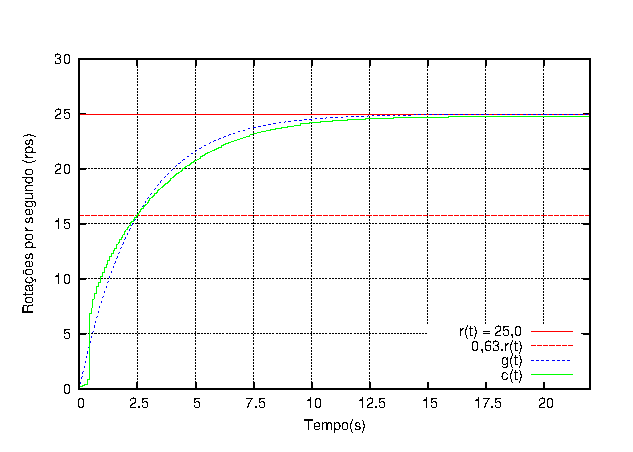
\includegraphics[scale=0.9]{./imagens/acaoMalhaAbertaTau.eps}
\label{fig:acaoMalhaAberTau}

%{\small Fonte: Próprio autor}
\end{figure}


\end{frame}


%%%%%%%%%%%%%%%%%%%%%%%%%%%%%%%%%%%%%%% Formato Canônico
\begin{frame}{Modelo do Sistema em Malha Aberta - Formato Canônico}

$  \frac{C(s)}{R(s)}=\frac{K}{s+a}=\frac{0,4}{s+0,4} $
\hspace{1cm}
$\frac{C(s)}{R(s)} = \frac{1}{\tau s+1} = \frac{1}{2,5 s+1} = g(t)$

\vspace{-0.5cm}
\begin{figure}[!htb]
%\caption{Ação de Controle em Malha Aberta}
\center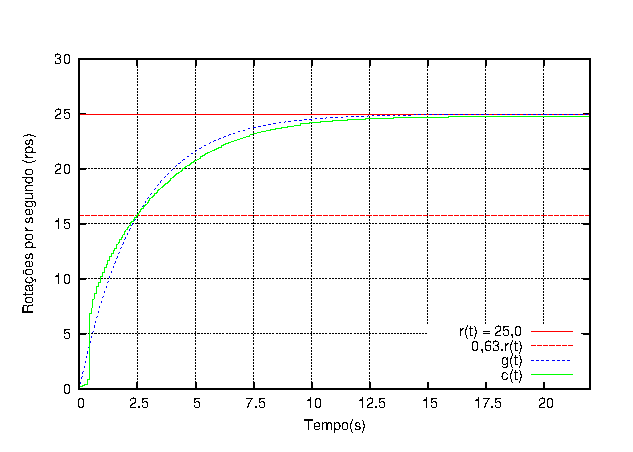
\includegraphics[scale=0.9]{./imagens/acaoMalhaAbertaTau.eps}
\label{fig:acaoMalhaAberTau}

%{\small Fonte: Próprio autor}
\end{figure}


\end{frame}



%%%%%%%%%%%%%%%%%%%%%%%%%%%%%%%%%%%%%%% Qualidade do Modelo
\begin{frame}{Qualidade do Modelo}
Erro Relativo Percentual

\begin{equation}
 \% erro = \frac{100}{N} . \sum_{n = 0,00}^{n=22,40} {\frac{| \text{\emph{r[n]}} -\text{\emph{c[n]}} |}{\text{\emph{r[n]}}} } 
\end{equation}

Onde:

\setlength{\parindent}{2cm}
r : valor real; 

c : valor calculado;

n : número da amostra aquisitada;

N : número total de amostras.


\end{frame}



%%%%%%%%%%%%%%%%%%%%%%%%%%%%%%%%%%%%%%% Qualidade do Modelo
\begin{frame}{Qualidade do Modelo}

\begin{table}[h]
\centering
\caption{Erro Relativo Percentual para intervalos determinados por $\tau$ }
\label{tab:ErroModeloTau}

\begin{tabular}{c|c}
\hline
Intervalo de amostras  &  erro médio relativo \\ \hline
\hline
%0 a 1 $\tau$ & 83,40 \% \\ \hline
1 a 2 $\tau$ &  3,16 \% \\ \hline
2 a 3 $\tau$ &  3,38 \% \\ \hline
3 a 4 $\tau$ &  2,00 \% \\ \hline
4 a 5 $\tau$ &  2,29 \% \\ \hline
$>$ 5 $\tau$ &  0,82 \% \\ \hline
\end{tabular}

%{\vspace{0.2cm} \small Fonte: Próprio autor}
\end{table}


\end{frame}



% Resultados
\section{Resultados}


%%%%%%%%%%%%%%%%%%%%%%%%%%%%%%%%%%%%%%% Implementação da LPA2v
\begin{frame}{Implementação da LPA2v}

\emph{ P:  eixo do motor apresenta rotação igual ao valor de referência.}

\begin{itemize}
\item $\mu _0$ : grau de evidência favorável que refere-se ao valor desejado;
\item $\mu _1$ : grau de evidência favorável com que o motor atinge a velocidade de rotação desejada;
\end{itemize}
O bloco LPA2v calcula os graus de evidência desfavoráveis das respectivas entradas:

\centering
$\lambda _0 = 1- \mu _0   \hspace{1cm}   \lambda _1 = 1 - \mu_1 $

\vspace{0.5cm}

Para o cálculo dos graus de Certeza e Contradição são utilizados:

\vspace{0.5cm}
\resizebox{!}{0.6cm}{ $ P _{(\mu_0, \lambda_1)} $}


\end{frame}









%%%%%%%%%%%%%%%%%%%%%%%%%%%%%%%%%%%%%%% Diagrama de blocos do Controle utilizando a LPA2v
\begin{frame}{Diagrama de blocos do Controle utilizando a LPA2v}

\begin{figure}[!h]
\centering
%\caption{Diagrama de blocos do controle utilizando a LPA2v}
\begin{tikzpicture}[scale=0.75]
\tikzset{ >=latex, inner sep=0pt, outer sep=0pt,  }

%\draw [lightgray, dashed](0,0) grid (15,7);

%%% Blocos 

% K normalização rps -> 0..1
\node [fill=black, circle] (KSP0) at (1,6.5) { };
\node [fill=black, circle] (KSP1) at (2,5.5) { };
\draw[thick] (KSP0) rectangle (KSP1);
\fill[white, nearly transparent] (KSP0) rectangle (KSP1);
\node [fill=black, circle] (KSPin)  at (1.0,6.0) { }; 
\node [fill=black, circle] (KSPout) at (2.0,6.0) { }; 
\node (Kn1) at (1.5,6.0) {$K_n$};

% K normalização  0..1 --> %PWM
\node [fill=black, circle] (KPWM0) at (4,6.5) { };
\node [fill=black, circle] (KPWM1) at (5,5.5) { };
\draw[thick] (KPWM0) rectangle (KPWM1);
\fill[white, nearly transparent] (KPWM0) rectangle (KPWM1);
\node [fill=black, circle] (KPWMin)  at (4.0,6.0) { };
\node [fill=black, circle] (KPWMout) at (5.0,6.0) { };
\node (K100) at (4.5,6.0) {$K_{\%}$};

% Planta
\node [fill=black, circle] (GT0) at (13,6.5) { };
\node [fill=black, circle] (GT1) at (14,5.5) { };
\draw[thick] (GT0) rectangle (GT1);
\fill[white, nearly transparent] (GT0) rectangle (GT1);
\node [fill=black, circle] (GTin)  at (13.0,6.0) { };
\node [fill=black, circle] (GTout) at (14.0,6.0) { };
\node (planta) at (13.5,6.0) {$g(t)$};

% Saturação
\node [fill=black, circle] (SAT0) at (11,6.5) { };
\node [fill=black, circle] (SAT1) at (12,5.5) { };
\draw[thick] (SAT0) rectangle (SAT1);
\fill[white, nearly transparent] (SAT0) rectangle (SAT1);
\node [fill=black, circle] (SATin)  at (11.0,6.0) { };
\node [fill=black, circle] (SATout) at (12.0,6.0) { };
\draw [thick] (11.2,5.7) -- (11.4,5.7) -- (11.6,6.3) -- (11.8,6.3);
\draw [gray, thick] (11.2,6.0) -- (11.8,6.0);
\draw [gray, thick] (11.5,5.7) -- (11.5,6.3);

% Multiplicacao
\node [fill=black, circle] (MUL0) at (8,4.5) { };
\node [fill=black, circle] (MUL1) at (9,2.5) { };
\draw[thick] (MUL0) rectangle (MUL1);
\fill[white, nearly transparent] (MUL0) rectangle (MUL1);
\node [fill=black, circle] (MULin0) at (8.0,4.0) { };
\node [fill=black, circle] (MULin1) at (8.0,3.0) { };
\node [fill=black, circle] (MULout) at (9.0,3.5) { };
\node (multi) at (8.5,3.5) {$x$};

% Klp
\node [fill=black, circle] (KLP0) at (6,3.5) { };
\node [fill=black, circle] (KLP1) at (7,2.5) { };
\draw[thick] (KLP0) rectangle (KLP1);
\fill[white, nearly transparent] (KLP0) rectangle (KLP1);
\node [fill=black, circle] (KLPin)  at (6.0,3.0) { };
\node [fill=black, circle] (KLPout) at (7.0,3.0) { };
\node (KLP) at (6.5,3.0) {$K_{LP}$};

% Sensor
\node [fill=black, circle] (KS0) at (6,1.5) { };
\node [fill=black, circle] (KS1) at (7,0.5) { };
\draw[thick] (KS0) rectangle (KS1);
\fill[white, nearly transparent] (KS0) rectangle (KS1);
\node [fill=black, circle] (KSin)  at (7.0,1.0) { };
\node [fill=black, circle] (KSout) at (6.0,1.0) { };
\node (Kn2) at (6.5,1.0) {$K_n$};

% LPA2v
\node [fill=black, circle] (LPA0) at (3,4.5) { };
\node [fill=black, circle] (LPA1) at (5,2.5) { };
\draw[thick] (LPA0) rectangle (LPA1);
\fill[white, nearly transparent] (LPA0) rectangle (LPA1);
\node [fill=black, circle] (LPAu0) at (3.0,4.0) { };
\node [fill=black, circle] (LPAu1) at (3.0,3.0) { };
\node [fill=black, circle] (LPAgc)  at (5.0,4.0) { };
\node [fill=black, circle] (LPAgct) at (5.0,3.0) { };
\draw [thick] (4.0,4.5) -- (5.0,3.5) -- (4.0,2.5) -- (3.0,3.5) -- (4.0,4.5);
\node (LPA2v) at (4.0,3.5) {$LPA2v$};
\draw [thick] (LPAgc) -- (5.3,4.0);
\node (LPA2vu0)  at (2.0,4.1) {$\mu _0$};
\node (LPA2vu1)  at (2.0,3.1) {$\mu _1$};
\node (LPA2vGc)  at (5.3,4.3) {$G_c$};
\node (LPA2vGct) at (5.3,3.3) {$G_{ct}$};


% Somador
\node [fill=black, circle] (SUM) at (9.5,6.0) { };
\filldraw[fill=white,thick] (SUM) circle (5mm);
\node [fill=black, circle] (SUMin0) at ( 9.0,6.0) { };
\node [fill=black, circle] (SUMin1) at ( 9.5,5.5) { };
\node [fill=black, circle] (SUMout) at (10.0,6.0) { };
\node (Sum0) at (9.2,6.0) {$+$};
\node (Sum1) at (9.5,5.7) {$+$};



%%% Linhas 

% set point
\draw [->, thick] (0.0,6.0) -- (KSPin);
\node (rt) at (0.5,6.3) {$r(t)$};

% setpoint -> normalização %PWM
\draw [->, thick] (KSPout) -- (KPWMin);

% normalização %PWM -> SUM
\draw [->, thick] (KPWMout) -- (SUMin0);

% SUM -> Saturação
\draw [->, thick] (SUMout) -- (SATin);

% Saturação -> GT
\draw [->, thick] (SATout) -- (GTin);

% GT -> fim
\draw [->, thick] (GTout) -- (15,6);
\node (ct) at (14.5,6.3) {$c(t)$};

% LPA2v Gct -> KLP
\draw [->, thick] (LPAgct) -- (KLPin);

% KLP -> MULin1
\draw [->, thick] (KLPout) -- (MULin1);

% normalização 0..1 -> LPA2v u0
\draw [->, thick] (2.5,6.0) -- (2.5,4.0) -- (LPAu0);

% normalização %PWM -> MULT in0
\draw [->, thick] (7.5,6.0) -- (7.5,4.0) -- (MULin0);

% MULT out -> SUM in1
\draw [->, thick] (MULout) -- (9.5,3.5) -- (SUMin1);

% Fim -> sensor
\draw [->, thick] (14.5,6.0) -- (14.5,1.0) -- (KSin);

% Sensor -> LPA u2
\draw [->, thick] (KSout) -- (2.5,1.0) -- (2.5,3.0) --(LPAu1);

\end{tikzpicture}
\label{fig:diagramaBlocosLPA2v}

%{\vspace{0.2cm} \small Fonte: Próprio autor}
\end{figure}


\end{frame}


%%%%%%%%%%%%%%%%%%%%%%%%%%%%%%%%%%%%%%% Descrição do diagrama
\begin{frame}{Descrição do diagrama de blocos}


\begin{itemize}
  \item $K_n$: Bloco de normalização: rps para um intervalo fechado entre 0,0 e 1,0;

  \item $K_{\%}$: Bloco de normaliza: intervalo fechado entre 0,0 e 1,0 para um intervalo de 0 a 100 (\%PWM);

  \item $LPA2v$: Calcula os graus de Certeza e Contradição 
de acordo com os graus de evidência favorável $\mu _0$ e $\mu _1$;

  \item $K_{LP}$: Coeficiente de ganho proporcional do grau de contradição;

  \item $x$: Bloco multiplicador;

  \item $g(t)$: Planta do sistema;

  \item $Soma$: Bloco somador;

  \item \emph{Saturação}: Bloco limitador, impede o valor do PWM ultrapassar seu valor máximo de 100\%. 
\end{itemize}



\end{frame}



%%%%%%%%%%%%%%%%%%%%%%%%%%%%%%%%%%%%%%% Ação de Controle utilizando LPA2v
\begin{frame}{Ação de Controle utilizando LPA2v}

\begin{figure}[!htb]
%\caption{Ação de controle utilizando LPA2v}
\vspace{-1cm}\center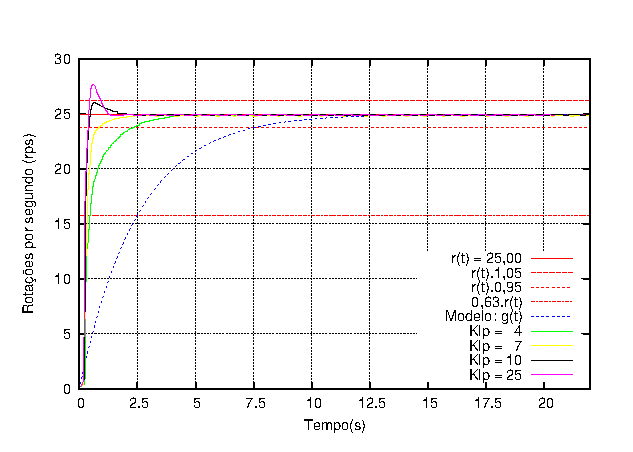
\includegraphics[scale=1.0]{./imagens/klpAll.eps}
\label{fig:acaoLPA2v}

%{\small Fonte: Próprio autor}
\end{figure}


\end{frame}



%%%%%%%%%%%%%%%%%%%%%%%%%%%%%%%%%%%%%%% Ação de Controle utilizando LPA2v
\begin{frame}{Ação de Controle utilizando LPA2v}


\begin{figure}[!htb]
%\caption{Ação de controle utilizando LPA2v para valores alvo variáveis}
\vspace{-1cm}
\center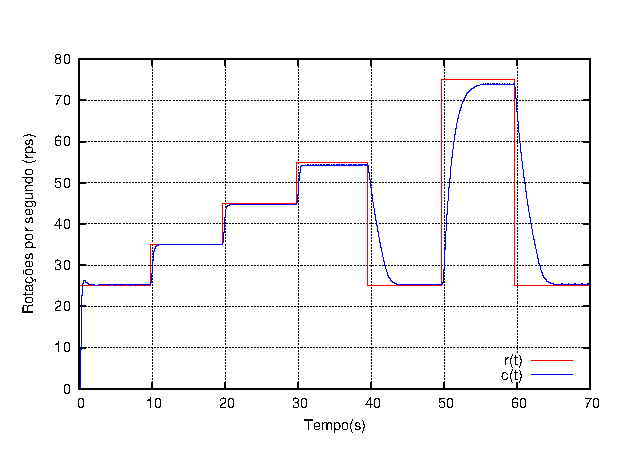
\includegraphics[scale=1.0]{./imagens/patam85.eps}
\label{fig:acaoLPA2vpatam85}

%{\small Fonte: Próprio autor}
\end{figure}

\end{frame}



% Conclusao
\section{Cronograma}

\begin{frame}{Cronograma}
\begin{enumerate}\small
  \item \label{LPA2v}       Entregar o estudo da LPA2v aplicada ao Controle de Sistemas.
  \item \label{controlar}   Entregar a implementação de um controlador utilizando LPA2v.
  \item \label{configurar}  Entregar a configuração do controlador.
  \item \label{descrever}   Entregar a descrição do controlador e dos parâmetros de ajuste.
  \item \label{otimizar1}   Entregar a primeira otimização dos parâmetros e analise da performance.
  \item \label{otimizar2}   Entregar a segunda otimização dos parâmetros e analisar a performance do controlador.
  \item \label{entregar}    Entregar a revisão de toda a dissertação.
  \item \label{finalizar}   Entregar a dissertação finalizada.
  \item \label{corrigir}    Entregar a correção da dissertação.
  \item \label{imprimir}    Entregar a impressão da dissertação.
  \item \label{finalApres}  Entregar a apresentação finalizada.
  \item \label{apresentar}  Apresentar a dissertação.
\end{enumerate}
\end{frame}



%%%%%%%%%%%%%%%%%%%%%%%%%%%%%%%%%%%%%%%
\begin{frame}{Cronograma }
\vspace{-1cm}
\begin{table}[t]
%\caption{Cronograma de atividades}
\begin{center}
\resizebox{\textwidth}{!}
{
  \begin{tabular}{c|l|l|l|l|l|l|l|l|l|l|l|l }
  \hline
  \multicolumn{1}{c|}
     {\multirow{2}{*}{Tarefas}} & 
     \multicolumn{2}{c|}{Jul} &
     \multicolumn{2}{|c|}{Ago} &
     \multicolumn{2}{|c|}{Set} & 
     \multicolumn{2}{|c|}{Out} &
     \multicolumn{2}{|c|}{Nov} &
     \multicolumn{2}{|c }{Dez} \\ \cline{2-13}
     \multicolumn{1}{ c|}{} & 12 & 26 & 16 & 30 & 13 & 27 & 11 & 25 & 15 & 29 & 06 & 13 \\ 
  \hline
  \hline
  %\rowcolor[HTML]{EFEFEF}
  \ref{LPA2v} 	  & \cellcolor{lightgray} &&&&&&&&&&&  \\ \hline
  \ref{controlar} && \cellcolor{lightgray} &&&&&&&&&&  \\ \hline
  \ref{configurar}&&& \cellcolor{lightgray} &&&&&&&&&  \\ \hline
  \ref{descrever} &&&& \cellcolor{lightgray} &&&&&&&&  \\ \hline
  \ref{otimizar1} &&&&& \cellcolor{gray} &&&&&&&  \\ \hline
  \ref{otimizar2} &&&&&& \cellcolor{gray} &&&&&&  \\ \hline
  \ref{entregar}  &&&&&&& \cellcolor{darkgray} &&&&&  \\ \hline
  \ref{finalizar} &&&&&&&& \cellcolor{darkgray} &&&&  \\ \hline
  \ref{corrigir}  &&&&&&&&& \cellcolor{darkgray} &&&  \\ \hline
  \ref{imprimir}  &&&&&&&&&& \cellcolor{darkgray} &&  \\ \hline
  \ref{finalApres}&&&&&&&&&& \cellcolor{darkgray} &&  \\ \hline
  \ref{apresentar}&&&&&&&&&&& \cellcolor{black} &  \\ \hline
  \hline
  \end{tabular}
}
\end{center}
%\label{tab:cronograma}
%\vspace{0.5cm}
\centering
%{\small Fonte: Próprio autor}
\end{table}

\end{frame}




%%%%%%%%%%%%%%%%%%%%%%%%%%%%%%%%%%%%%%%
\section{Viabilidade}


\begin{frame}{Viabilidade Econômica}
Custo dos itens adquiridos para montagem do projeto
\small
\begin{table}[h]
\centering
%\caption{Custo dos itens adquiridos para montagem do projeto}
\label{tab:custos}
\begin{tabular}{c|c|c}
\hline
Item  & Descrição  & Valor \\ \hline
\hline
1 & Placa de desenvolvimento modelo Tiva$ ^{TM}$ TM4C123G & $R\$ 42,00 $ \\ \hline
2 & Placa padrão perfurada 10x15 cm & $R\$ 15,00 $ \\ \hline
3 & Componentes eletrônicos diversos & $R\$20,00$ \\ \hline
4 & Fonte de alimentação & $R\$60,00 $ \\ \hline
\hline
  & Total & $R\$137,00 $ \\ \hline
\hline
\end{tabular}

%{\vspace{0.4cm} \small Fonte: Próprio autor}
\end{table}


\end{frame}






%%%%%%%%%%%%%%%%%%%%%%%%%%%%%%%%%%%%%%%
\begin{frame}{Viabilidade Econômica}
Itens que não geraram custo direto ao projeto
\begin{table}[h]
\centering
%\caption{Itens que não geraram custo direto ao projeto}
\label{tab:equipamentos}
\begin{tabular}{c|c}
\hline
Item  & Descrição \\ \hline
\hline
1 & Microcomputador portátil - Notebook \\ \hline
2 & Softwares  \\ \hline
3 & Multímetro \\ \hline
4 & Motor CC \\ \hline
5 & Disco acoplado ao motor \\ \hline
\hline
\end{tabular}

%{\vspace{0.4cm} \small Fonte: Próprio autor}
\end{table}

\end{frame}





%%%%%%%%%%%%%%%%%%%%%%%%%%%%%%%%%%%%%%%
\begin{frame}{Viabilidade Econômica}

Ferramentas de uso livre 
\begin{itemize}
\item Sistema Operacional: GNU/Linux Debian 8(Jessie);
\item GNOME Shell;
\item Editor de texto e códigos fonte VIM;
\item compilador GCC para ARM (arm-none-eabi-gcc);
\item GNU Make;
\item processador de texto \LaTeX - pdfTEX;
\item pacotes geradores de figuras TikZ, PGF e GNU pic(Groff);
\item gerador de gráficos GNUPlot;
\item teminal de comunicação Minicom;
\item gravador LM4Flash.
\end{itemize}

\end{frame}



% Referencias
\section{Referencias}
\begin{frame}{Referências}
%	\bibliographystile{abnt-num}
\small
	\bibliography{bib/bibliografia}
\end{frame}


% Agradecimentos
\section{}
  \begin{frame}{Agradecimentos}
    \begin{figure}[!htb]
      \center
\includegraphics[scale=0.6]{./figuras/logo_IFSP.jpg}
    \end{figure}

    \centering

    \vspace{1cm}
    Agradeço a todos!
	
  \end{frame}

\end{document}
